\section{Exercise 1} \label{P1}
% Write some intro
\textit{[Comment] For the last exercises include an image of the initial robot image of the final robot configuration} 

\textit{[Comment] For each exercise report the results obtained and provide an explanation of the result obtained (even though it might seem trivial). The matlab code is NOT an explanation of the algorithm.}
 
\subsection{Q1.1}
\label{subsec::q11}
Given the ease of representation and comprehension of serial chain pose, it is crucial to compute the transformation matrices for each joint with respect to the preceding one. For instance, the transformation matrices $^i_jT_0$ in the initial configuration ($\mathbf{q}_0 = \mathbf{q} = \mathbf{0}_{1 \times 7}$) represent the transformation from frame $<i>$ with respect to the next consecutive frame $<j>$. It takes into account both the rotational and translational contributions:
\begin{itemize}
	\item The rotational contribution is computed with \textit{Yaw-Pitch-Roll} convention for rotation, which defines the sequence of rotations around the $z$, $y$, and $x$ axes, respectively;
	\item The translational contribution is represented by the elements contained in the first three rows of the last column of the transformation matrix.
\end{itemize}
It’s crucial to emphasize that these matrices vary based on the values of the vector $\mathbf{q}$ that contain values for uniquely determining each joint’s configuration.
Given the general form of the transformation matrix:
\begin{equation}
	^i_j T = \begin{pmatrix}
		^i_j R & ^i P_j \\
		\mathbf{0}_{1\times3} & 1
	\end{pmatrix}
\end{equation}
where $j$ is the considered chain's joint and $i$ is the joint with respect is considered the transformation, $^i_j R$ is the rotation matrix that define the rotation from the frame $<i>$ to $<j>$, and $^i_j P$ is the position of the frame $<j>$ with respect to frame $<i>$.
Taking into account $\mathbf{q} = \mathbf{0}_{1 \times 7}$ the transformation matrices for the initial configuration of the chain are:
\begin{align*}
	% Transformation matrix b to 1
	&^b_1 T_0 = \begin{pmatrix}
		1 & 0 & 0 & 0 \\
0      & 1 & 0 & 0 \\
0      & 0 & 1 & 0.105 \\
0      & 0 & 0 & 1
	\end{pmatrix} \quad
	% Transformation matrix 1 to 2
	^1_2 T_0 = \begin{pmatrix}
		0 & 1 & 0 & 0 \\
		0 & 0 & 1 & 0 \\
		1 & 0 & 0 & 0.110 \\
		0 & 0 & 0 & 1
	\end{pmatrix} \quad
	% Transformation matrix 2 to 3
	^2_3 T_0 = \begin{pmatrix}
		0 & 0 & 1 & 0.100 \\
		0 & -1 & 0 & 0 \\
		1 & 0 & 0 & 0 \\
		0 & 0 & 0 & 1
	\end{pmatrix} \quad
	% Transformation matrix 3 to 4
	^3_4 T_0 = \begin{pmatrix}
		0 & 0 & 1 & 0 \\
		0 & -1 & 0 & 0 \\
		1 & 0 & 0 & 0.325 \\
		0 & 0 & 0 & 1
	\end{pmatrix}
	\\
	% Transformation matrix 4 to 5
	&^4_5 T_0 = \begin{pmatrix}
		0 & 0 & 1 & 0.095 \\
		-1 & 0 & 0 & 0\\
		0 & -1 & 0 & 0\\
		0 & 0 & 0 & 1
	\end{pmatrix} \quad
	% Transformation matrix 5 to 6
	^5_6 T_0 = \begin{pmatrix}
		-1 & 0 & 0 & 0 \\
		0 & -1 & 0 & 0 \\
		0 & 0 & 1 & 0.095 \\
		0 & 0 & 0 & 1
	\end{pmatrix} \quad
	% Transformation matrix 6 to e
	^6_e T_0 = \begin{pmatrix}
		1 & 0 & 0 & 0 \\
		0 & 1 & 0 & 0 \\
		0 & 0 & 1 & 0.355 \\
		0 & 0 & 0 & 1
	\end{pmatrix}
\end{align*}

where:
\begin{itemize}
	\item $^b_1 T_0$ describes solely a translation along the $x$ axis of $0.105\,m$, then $^b_1 R_0 = \mathbf I_{3 \times 3}$ and $^b P_1 = (0,\,0,\,0.105)^T$;
	\item $^1_2 T_0$ represents two $\frac{\pi}{2}$ rotations, one around $z$ and one other around $y$, both clockwise. There is also a translation component along the $z$ axis of $0.110\,m$, then $^1_2 R_0 = R_z(-\frac{\pi}{2}) \cdot R_y(-\frac{\pi}{2})$ and $^1 P_2 = (0,\,0,\,0.110)^T$;
	\item $^2_3 T_0$, as $^1_2 T_0$, has two clockwise rotations around $z$ of $\pi$ and $y$ of $\frac{\pi}{2}$ and a translation along $x$ of $0.100\,m$. Formally it means $^2_3 R_0 = R_z(-\pi) \cdot R_y(-\frac{\pi}{2})$ and $^2 P_3 = (0.100,\,0,\,0)^T$;
	\item $^3_4 T_0$ describes an counterclockwise rotations around $z$ of $\pi$ and a clockwise rotation$y$ of $\frac{\pi}{2}$ and a translation along $z$ of $0.325\,m$. Formally it means $^3_4 R_0 = R_z(\pi) \cdot R_y(-\frac{\pi}{2})$ and $^3 P_4 = (0,\,0,\,0.325)^T$;
	\item $^4_5 T_0$ represents two clockwise rotations around $z$ and $x$ of $\frac{\pi}{2}$ and a translation along $x$ of $0.325\,m$. Formally it means $^4_5 R_0 = R_z(-\frac{\pi}{2}) \cdot R_y(-\frac{\pi}{2})$ and $^4 P_5 = (0.095,\,0,\,0)^T$;
	\item $^5_6 T_0$ express a counterclockwise rotation around $z$ of $\pi$ and a translation along $z$ of $0.095\,m$. Then $^5_6 R_0 = R_z(\pi)$ and $^5 P_6 = (0,\,0,\,0.095)^T$;
	\item $^6_e T_0$ highlight the presence of a translation along $z$ of $0.335\,m$. Then $^6_e R_0 = \mathbf I_{3 \times 3}$ and $^6 P_e = (0,\,0,\,0.335)^T$.
\end{itemize}

\subsection{Q1.2}
When the chain's pose changes a good method to update the initial configuration is through the transformation matrix:
\begin{equation}
	{}^i_j T = {}^i_j T_0 \cdot T_{\text{joint},\,j}
\end{equation}
where $^i_j T$ is defined as the transformation matrix for the new pose, and $T_{\text{joint},\,j}$ is the transformation matrix that accounts for the joint’s change of configuration:
\begin{equation}
	T_{\text{joint},\,j} = \begin{pmatrix}
		R_{z}(q_{j}) & P_j(q_{j}) \\
		\mathbf{0_{1x3}} & 1
	\end{pmatrix}
\end{equation}
The joint $j$, since the $z$ axis is defined coinciding with the joint's rotation axis, can either rotates $R_{z}(q_{j})$ or translates $P_{z}(q_{j})$ along $z$ on whether it is:
	\begin{itemize}
		\item A rotational joint: Only the rotational part of the transformation matrix contribute to the new configuration. The rotation is along along the $z$-axis and the new $T_{\text{joint},\,j}$ is:
		\begin{equation*}
			T_{\text{joint},\,j} = \begin{pmatrix}
				\cos(q_j) & -\sin(q_j) & 0 & 0 \\
				\sin(q_j) & \cos(q_j) & 0 & 0 \\
				0 & 0 & 1 & 0 \\
				0 & 0 & 0 & 1 \\
			\end{pmatrix} 
		\end{equation*}
		\item A translational joint: In this case, there is only a translation along the $z$-axis, then $T_{\text{joint},\,j}$ becomes:
		\begin{equation*}
		T_{\text{joint},\,j} = \begin{pmatrix}
			1 & 0 & 0 & 0 \\
			0 & 1 & 0 & 0 \\
			0 & 0 & 1 & q_j \\
			0 & 0 & 0 & 1 \\
		\end{pmatrix} 
		\end{equation*}
	\end{itemize}
For instance, given the vector $\mathbf{q} = (\frac{\pi}{4},\,-\frac{\pi}{4},\,0,\,-\frac{\pi}{4},\,0,\,0.150,\,\frac{\pi}{4})$, the updated transformation matrices $^i_j T$ are: 
\begin{gather*}
	^b_1 T = \begin{pmatrix}
		0.7071 & -0.7071 & 0 & 0 \\
		0.7071 & 0.7071 & 0 & 0 \\
		0 & 0 & 1 & 0.1050 \\
		0 & 0 & 0 & 1
	\end{pmatrix} \quad
	^1_2 T = \begin{pmatrix}
		-0.7071 & 0.7071 & 0 & 0 \\
		0 & 0 & 1 & 0 \\
		0.7071 & 0.7071 & 0 & 0.1100 \\
		0 & 0 & 0 & 1
	\end{pmatrix} \quad
	\quad ^2_3 T = \begin{pmatrix}
		0 & 0 & 1 & 0.1000 \\
		0 & -1 & 0 & 0 \\
		1 & 0 & 0 & 0 \\
		0 & 0 & 0 & 1
	\end{pmatrix} \\
	^3_4 T = \begin{pmatrix}
		0 & 0 & 1 & 0 \\
		0.7071 & -0.7071 & 0 & 0 \\
		0.7071 & 0.7071 & 0 & 0.3250 \\
		0 & 0 & 0 & 1
	\end{pmatrix} \quad
	\quad \quad ^4_5 T = \begin{pmatrix}
		0 & 0 & 1 & 0.0950 \\
		-1 & 0 & 0 & 0 \\
		0 & -1 & 0 & 0 \\
		0 & 0 & 0 & 1
	\end{pmatrix} \quad
	^5_6 T = \begin{pmatrix}
		-1 & 0 & 0 & 0 \\
		0 & -1 & 0 & 0 \\
		0 & -0 & 1 & 0.2450 \\
		0 & 0 & 0 & 1
	\end{pmatrix} \quad \\
	\\
	^6_e T = \begin{pmatrix}
		0.7071 & -0.7071 & 0 & 0 \\
		0.7071 & 0.7071 & 0 & 0 \\
		0 & 0 & 1 & 0.3550 \\
		0 & 0 & 0 & 1
	\end{pmatrix} \quad
	\nonumber
\end{gather*}
\begin{itemize}
	\item $^b_1 T$, where $q_1 = \frac{\pi}{4}$, represent only a counterclockwise rotation around the $z$-axis with respect to initial configuration. The result can be verified by comparing the new matrix $^1_b T$ with $^b_1 T_{0}$ in Subsection \ref{subsec::q11}. It is evident that there is a variation of the $R_{z}(q_1)$ component, while $P_{z}(q_1)$ remains unchanged;
	\item $^1_2 T$, as in the previous case, has $R_{z}(q_2)$ contribute to the new configuration, while the translational part remains unchanged;
	\item $^2_3 T$, since $q_3$ is zero, the configuration remains unchanged. It is evident that $^2_3 T = {}^2_3 T_{0}$; 
	\item $^3_4 T$ reflects that $q_4 = -\frac{\pi}{4}$. Indeed, there is only a rotational contribution along the $z$-axis and no translation;
	\item $^4_5 T$ similar to $^2_3 T$, is due to $q_5$ equals zero. Consequently, no rotations or variations take place. The resulting matrix is equivalent to the initial matrix, $^4_5 T_{0}$;
	\item $^5_6 T$ exhibits a translational contribution, on account of $q_6 = 0.15$. The rotational component of the matrix remains unchanged from the initial configuration. However, $P_{z}(q_6)$ is modified due to the translation along the $z$-axis.
	\item $^6_7 T$ shows, coherently with $q_7 = \frac{\pi}{4}$, a rotation around the $z$-axis. This means that the translational part, $P_{z}(q_7)$, remains unchanged. As result, the new transformation matrix $^6_7 T$ will differ from the initial configuration matrix $^6_7 T_{0}$ only in its rotational component.
\end{itemize}

\subsection{Q1.3}
The computation of the transformation matrices from the base frame $<b>$ to a given frame $<i>$ is directly governed by the following property:
\begin{equation}
	^b_e T = \prod_{j=1}^{e}\, {}^{i}_{j} T\Big\vert _{i=j-1}
\end{equation}
where generally the base frame $<b>$ has the value $i=0$. For instance, it is possible to compute $^b_e T$ for the new transformation matrices:
\begin{equation*}
		^b_e T = \begin{pmatrix}
		-0.5000 & -0.5000 & -0.7071 & -0.7039\\
		0.5000 & 0.5000 & -0.7071 & -0.7039 \\
		0.7071 & -0.7071 & 0 & 0.5155 \\
		0 & 0 & 0 & 1 \\
		\end{pmatrix}
\end{equation*}
or, applying the property $^i_j T = {}^k_i T^{-1} \cdot {}^k_j T$ it is possible to compute
\begin{equation*}
	^5_3 T = \begin{pmatrix}
		0 & 0.7071 & -0.7071 & 0.2298 \\
		-1 & 0 & 0 & 0\\
         0 & 0.7071 & 0.7071 & -0.3248 \\
         0 & 0 & 0 & 1
         \end{pmatrix}
\end{equation*}

\subsection{Q1.4}
The Jacobian matrix of the manipulator’s end-effector, which derives from a specified geometric model, comprises two distinct components: an angular contribution matrix $^b J^A_{e}$ and a linear contribution matrix $^b J^L_{e/b}$.
It is defined as:
\begin{equation}
	\renewcommand{\arraystretch}{1.5}
	^b J_{e/b} = \begin{pmatrix}
		^b J^A_{e} \\ 
		^b J^L_{e/b}
	\end{pmatrix}
\end{equation}
	These contributions are computed based on the type of joint considered (i.e., prismatic or rotational), using the following relationships:
	\begin{equation}
		^bJ_{e}^A =
		\begin{cases}
			{}^b k_{z} \quad &\text{for rotational joint}\\
			\mathbf{0} \quad &\text{for prismatic joint}
		\end{cases} \quad
		{}^bJ_{e/b}^L =
		\begin{cases}
			{}^b (k_{z} \times r_{e/b})  \quad &\text{for rotational joint}\\
			{}^b k_{z} \quad &\text{for prismatic joint}
		\end{cases}
	\end{equation}
where $\mathbf{k_{z}}$ is the unit vector along the joint axis (i.e., the $z$-axis, as the $z$ axis coincides with the joint's rotation axis), and $r_{e/b}$ is the position vector from the base to the end-effector. Notice that ${}^b r_{e/b} = {}^b_j T \cdot (0,\,0,\,0,\,1)^T$, then the Jacobian for the manipulator’s end-effector given $\mathbf{q} = (\frac{\pi}{4},\,-\frac{\pi}{4},\,0,\,-\frac{\pi}{4},\,0,\,0.150,\,\frac{\pi}{4})$ is:
\begin{equation*} 
	^b J_{e/b} = \begin{pmatrix}
		0 & 0 & 0 & 0 & 0 & 0 & 0\\
		0 & 0 & 0 & 0 & 0 & 0 & 0\\
		1 & 1 & 1 & 1 & 1 & 0 & 1 \\ 
		0 & 0 & 0.0500 & 0.2125 & 0.2797 & 0 & 0.7039 \\
		0 & 0 & -0.0500 & -0.2125 & -0.2797 & 0 & -0.7039 \\
		0 & 0 & 0 & 0 & 0 & 1 & 0\\
	\end{pmatrix}
\end{equation*}

 As evidence of the validity of the methods described thus far, a movement simulation is provided, see Figure \ref{fig::MotionOfTheManipulator}. The serial chain movement commences with configuration $\mathbf{q}_i = (\frac{\pi}{4},\,-\frac{\pi}{4},\,0,\,-\frac{\pi}{4},\,0,\,0.150,\,\frac{\pi}{4})$ and terminates with configuration $\mathbf{q}_f = (\frac{\pi}{4}+\frac{\pi}{6},\,-\frac{\pi}{4},\,0,\,-\frac{\pi}{4},\,0,\,0.150,\,\frac{\pi}{4})$, as depicted in Figure \ref{fig::FinalConfiguration}. This means that the first joint rotate counterclockwise around $z$-axis of $\frac{\pi}{6}$ with respect to $q_{i,\,1}$ as shown in Figure \ref{fig::MotionOfTheManipulator_top}.
 
 \begin{figure}
	\centering
	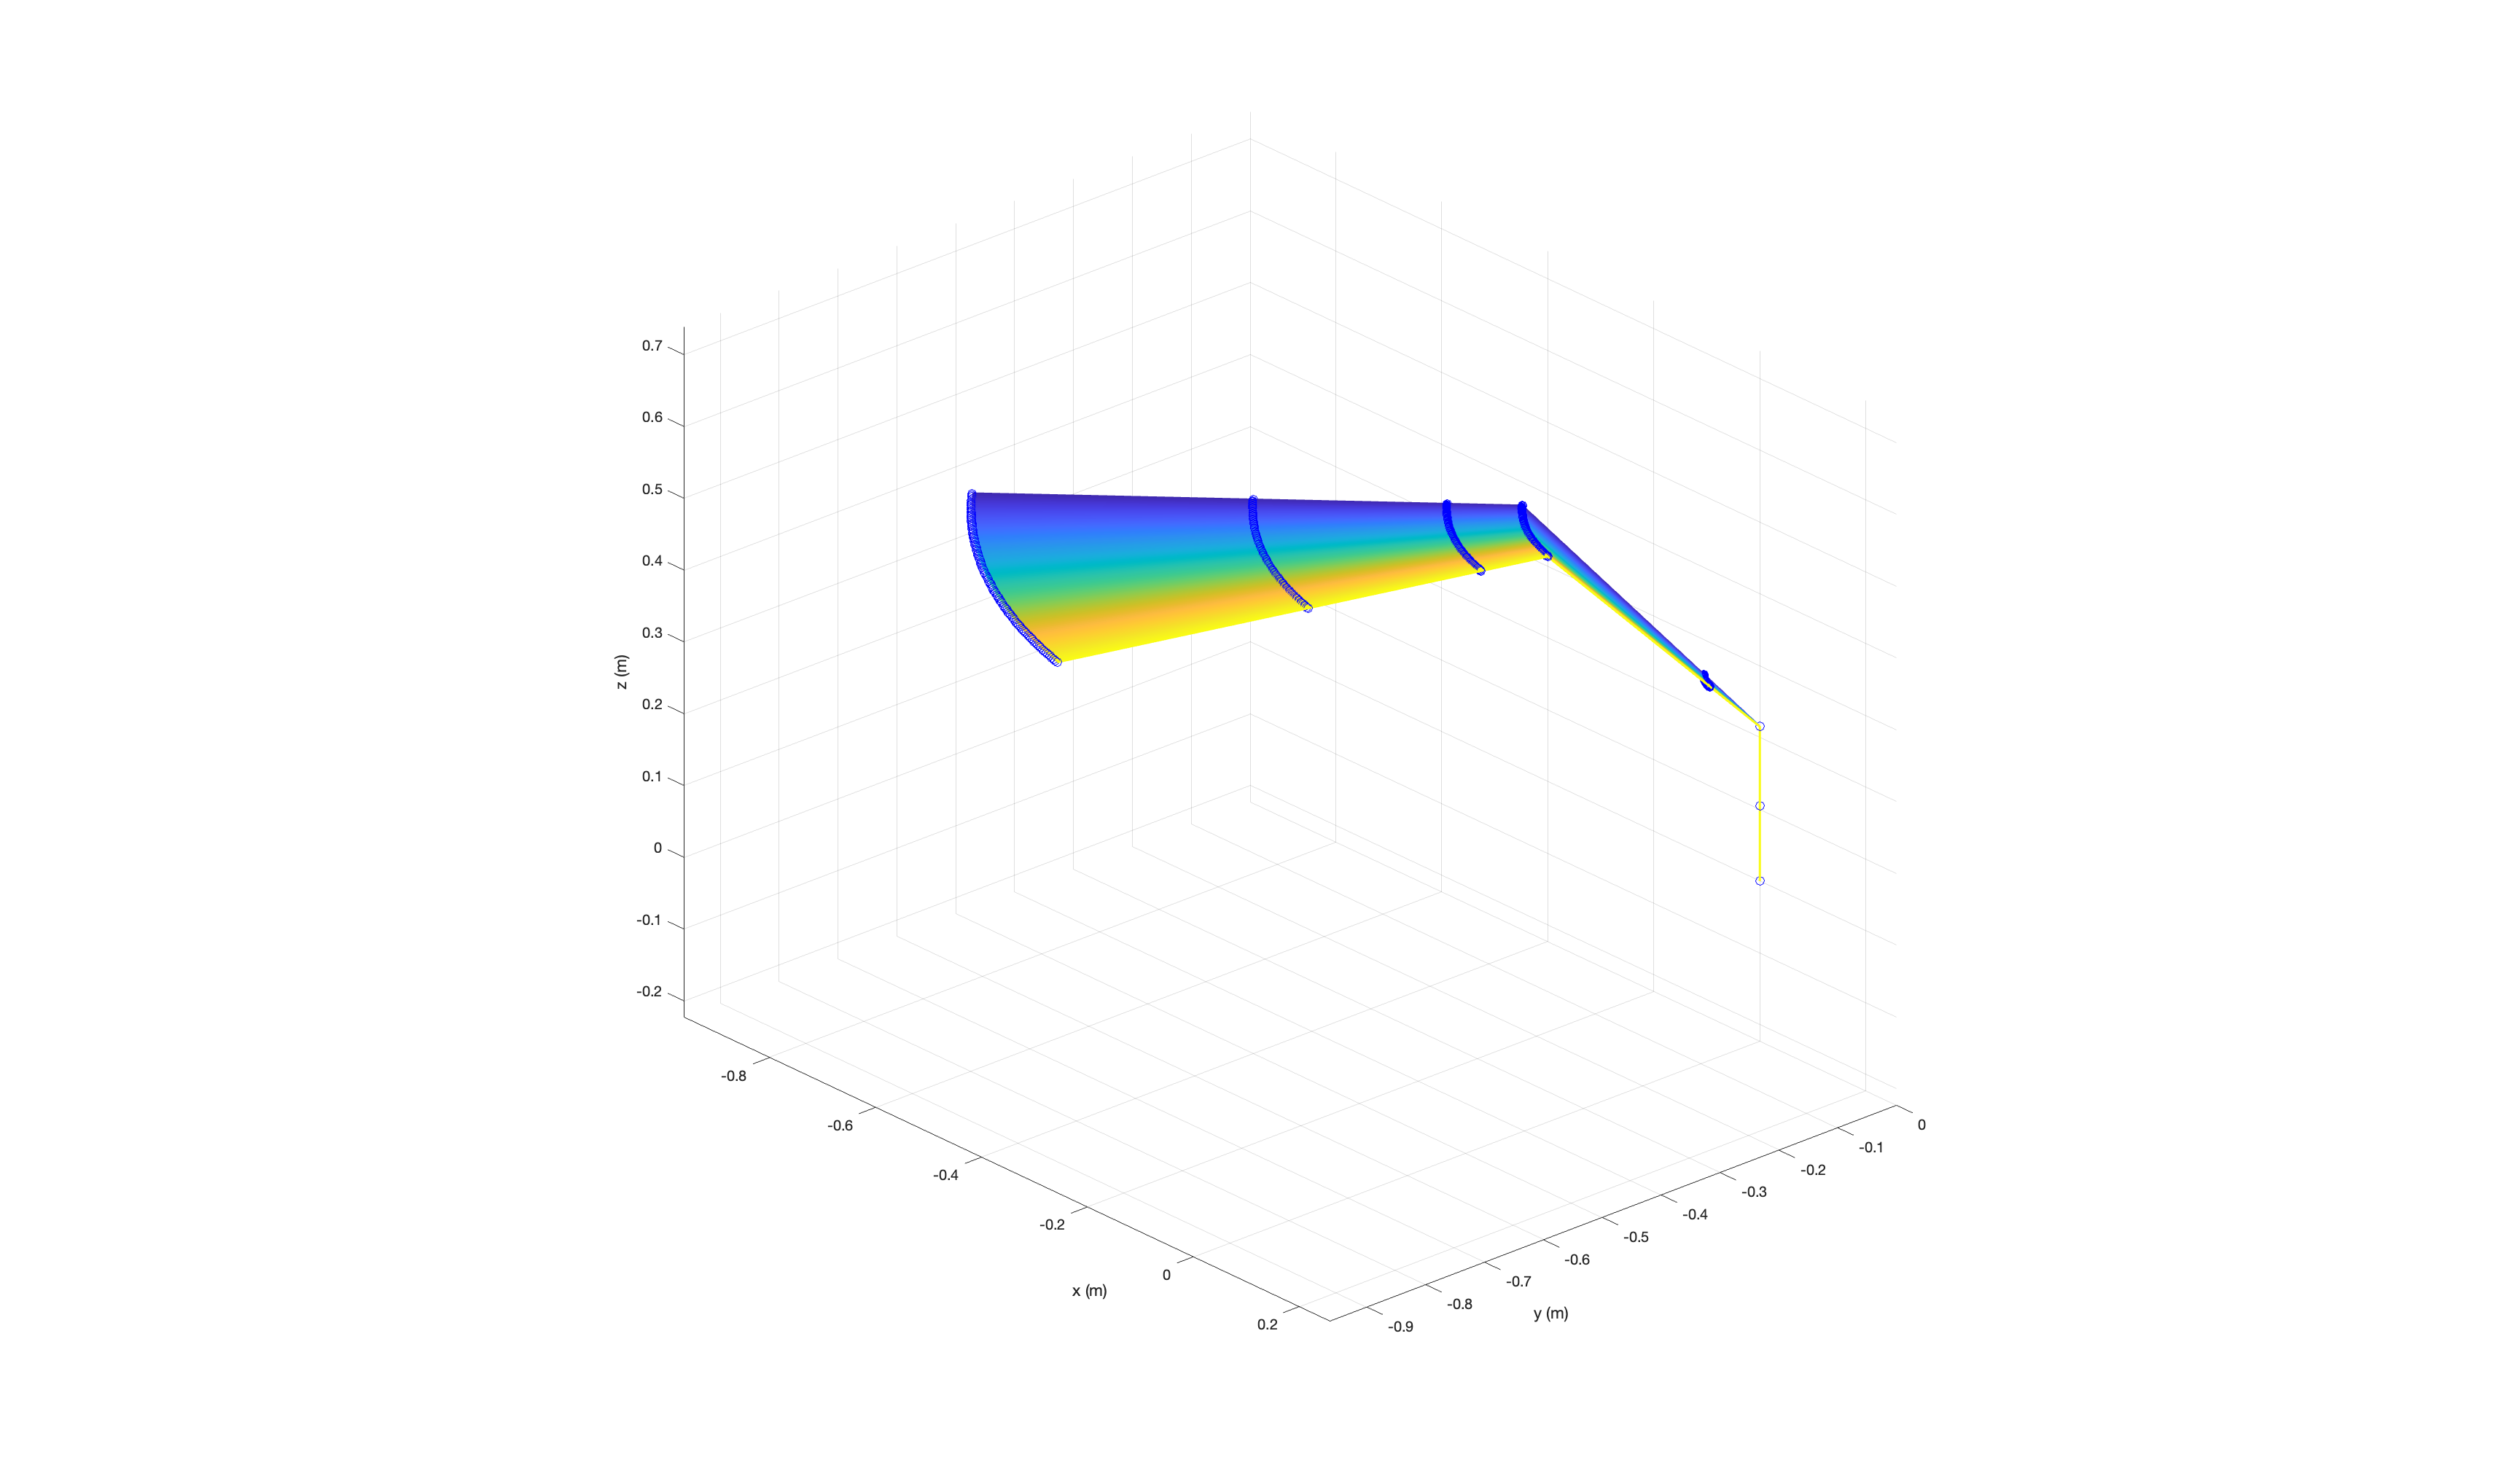
\includegraphics[width=0.75\textwidth]{Resources/MotionOfTheManipulator}
	\caption{Description of the manipulator’s simulation motion in a three-dimensional graph. The horizontal axes, denoted by $x$ and $y$, represent the horizontal motion, while the vertical axis, denoted by $z$, represents the vertical motion. The measurement units for all three axes are meters.}
	\label{fig::MotionOfTheManipulator}
\end{figure}
\begin{figure}
	\centering
	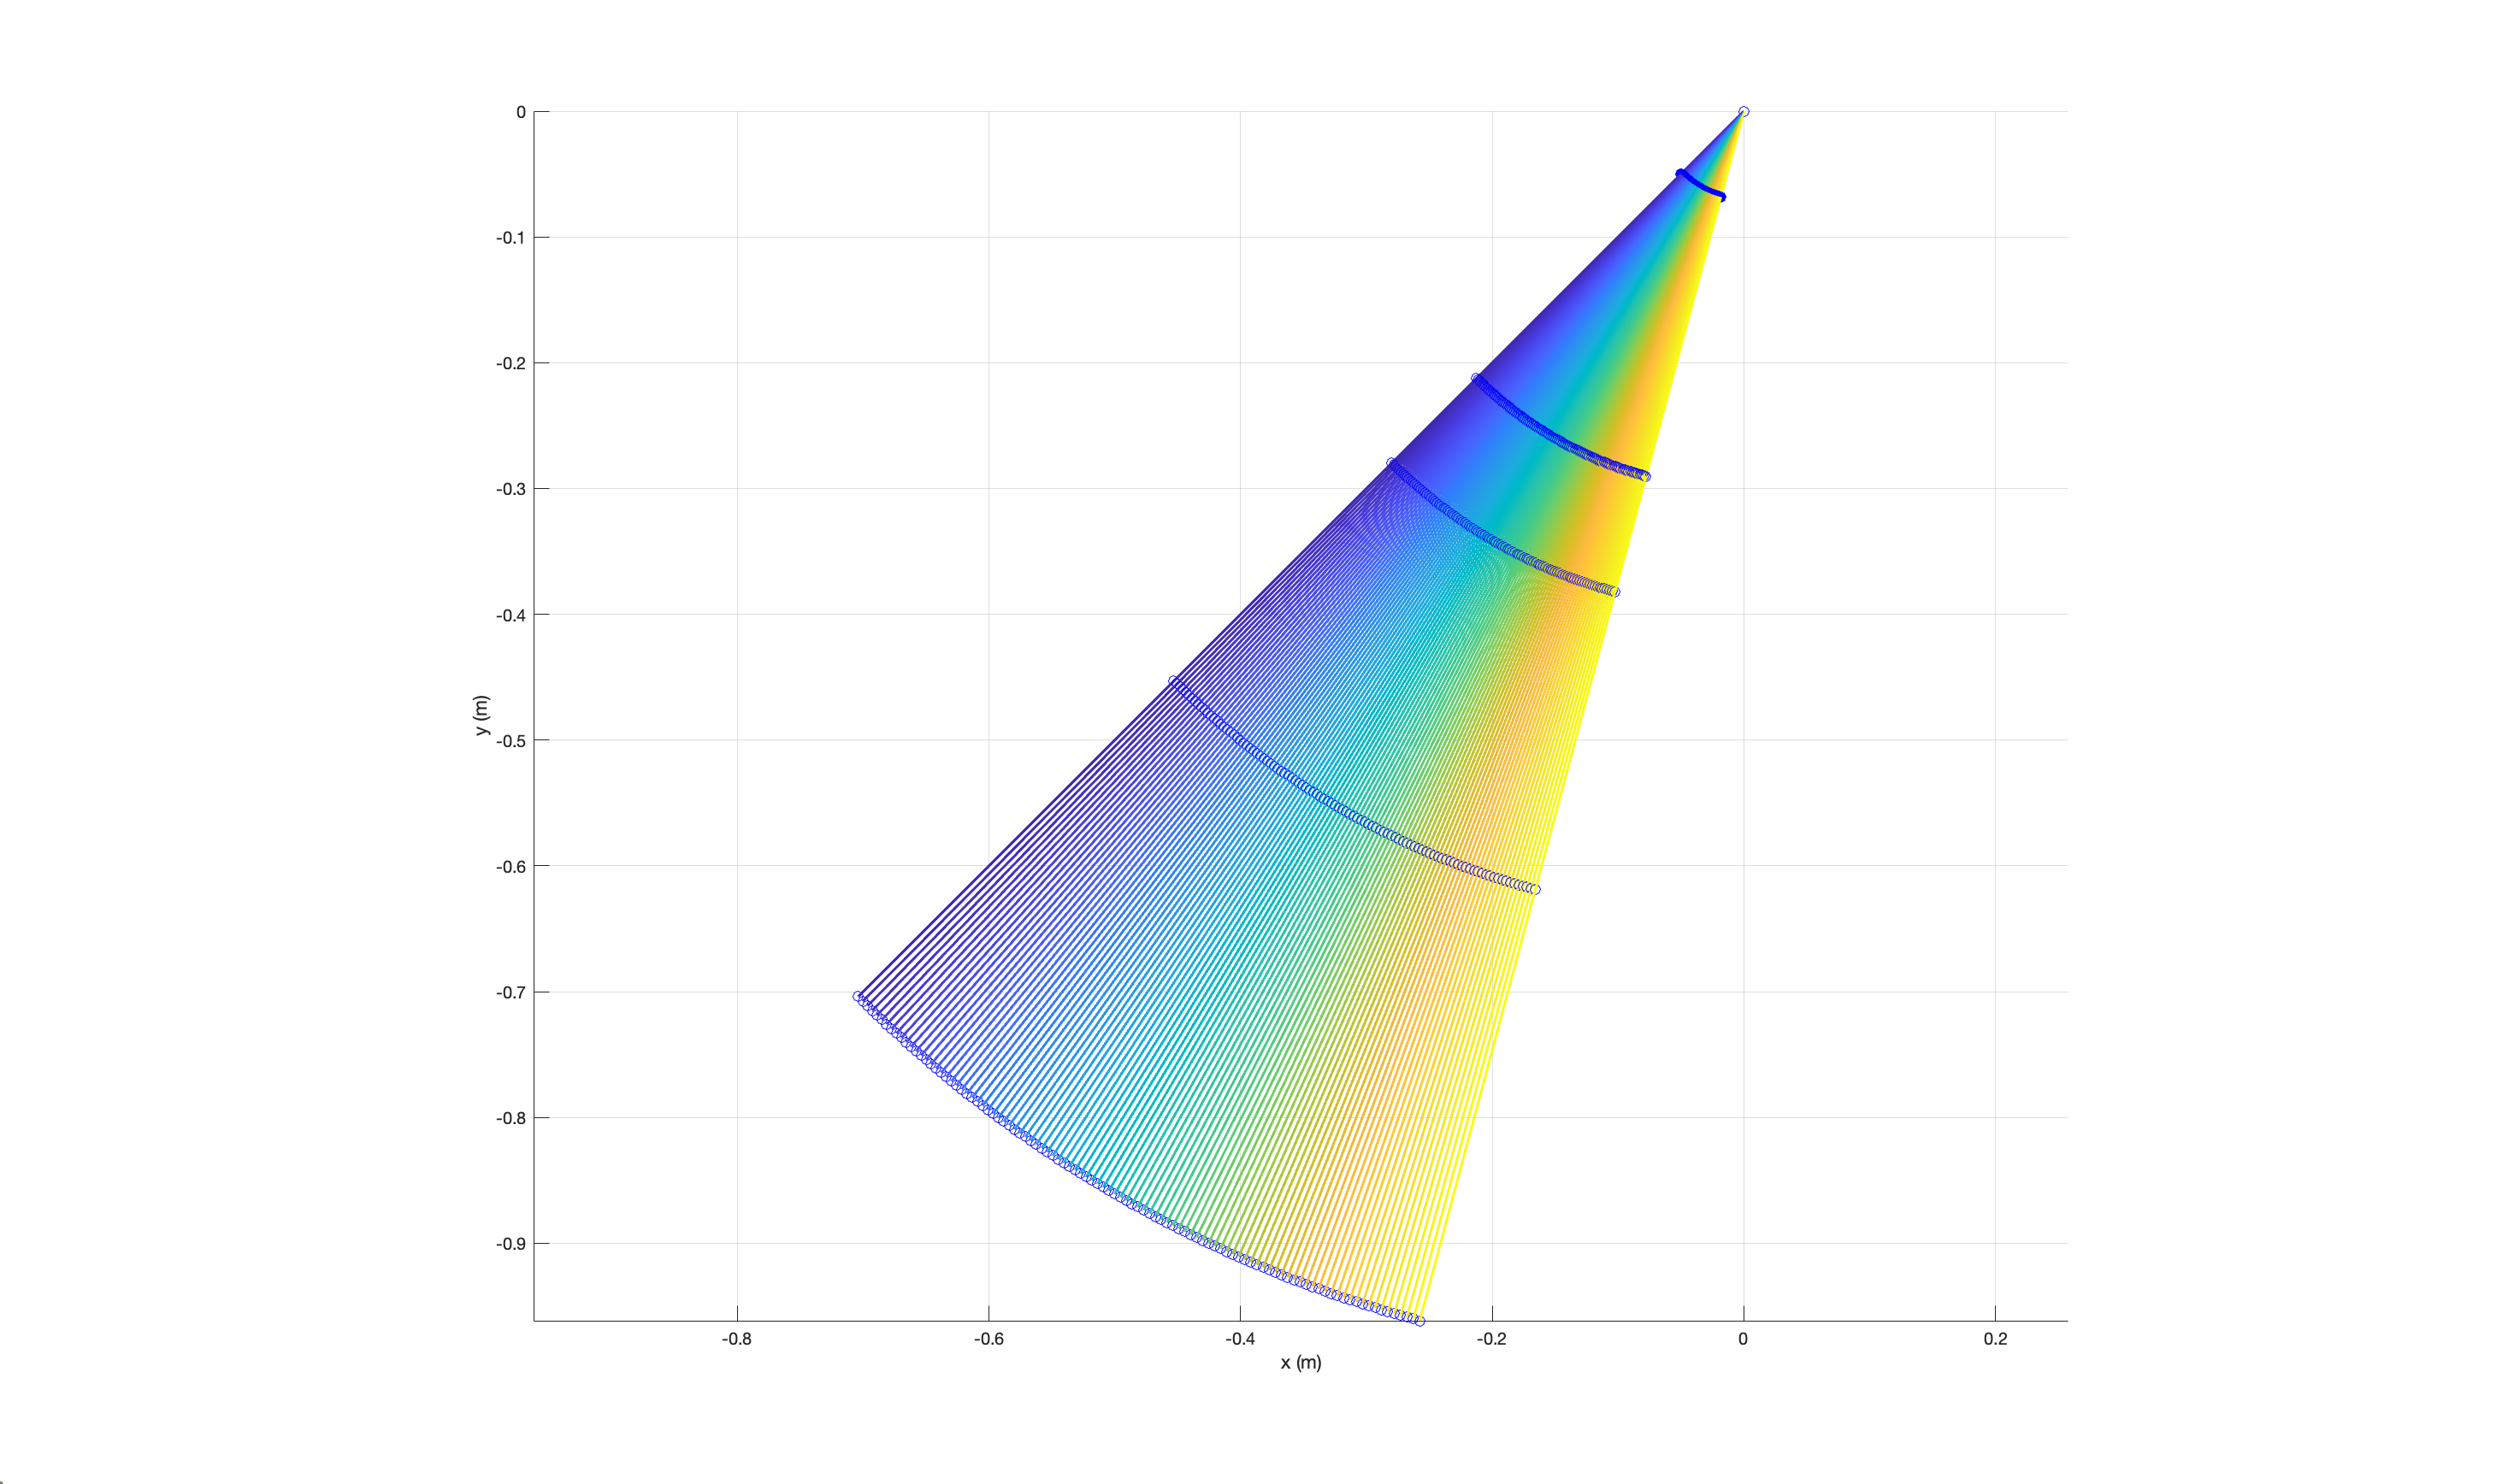
\includegraphics[width=0.75\textwidth]{Resources/MotionOfTheManipulator_top}
	\caption{Representation of the manipulator’s simulated motion on the Cartesian plane $(x, y)$. The measurement units for the three axes are meters.}
	\label{fig::MotionOfTheManipulator_top}
\end{figure}
\begin{figure}
	\centering
	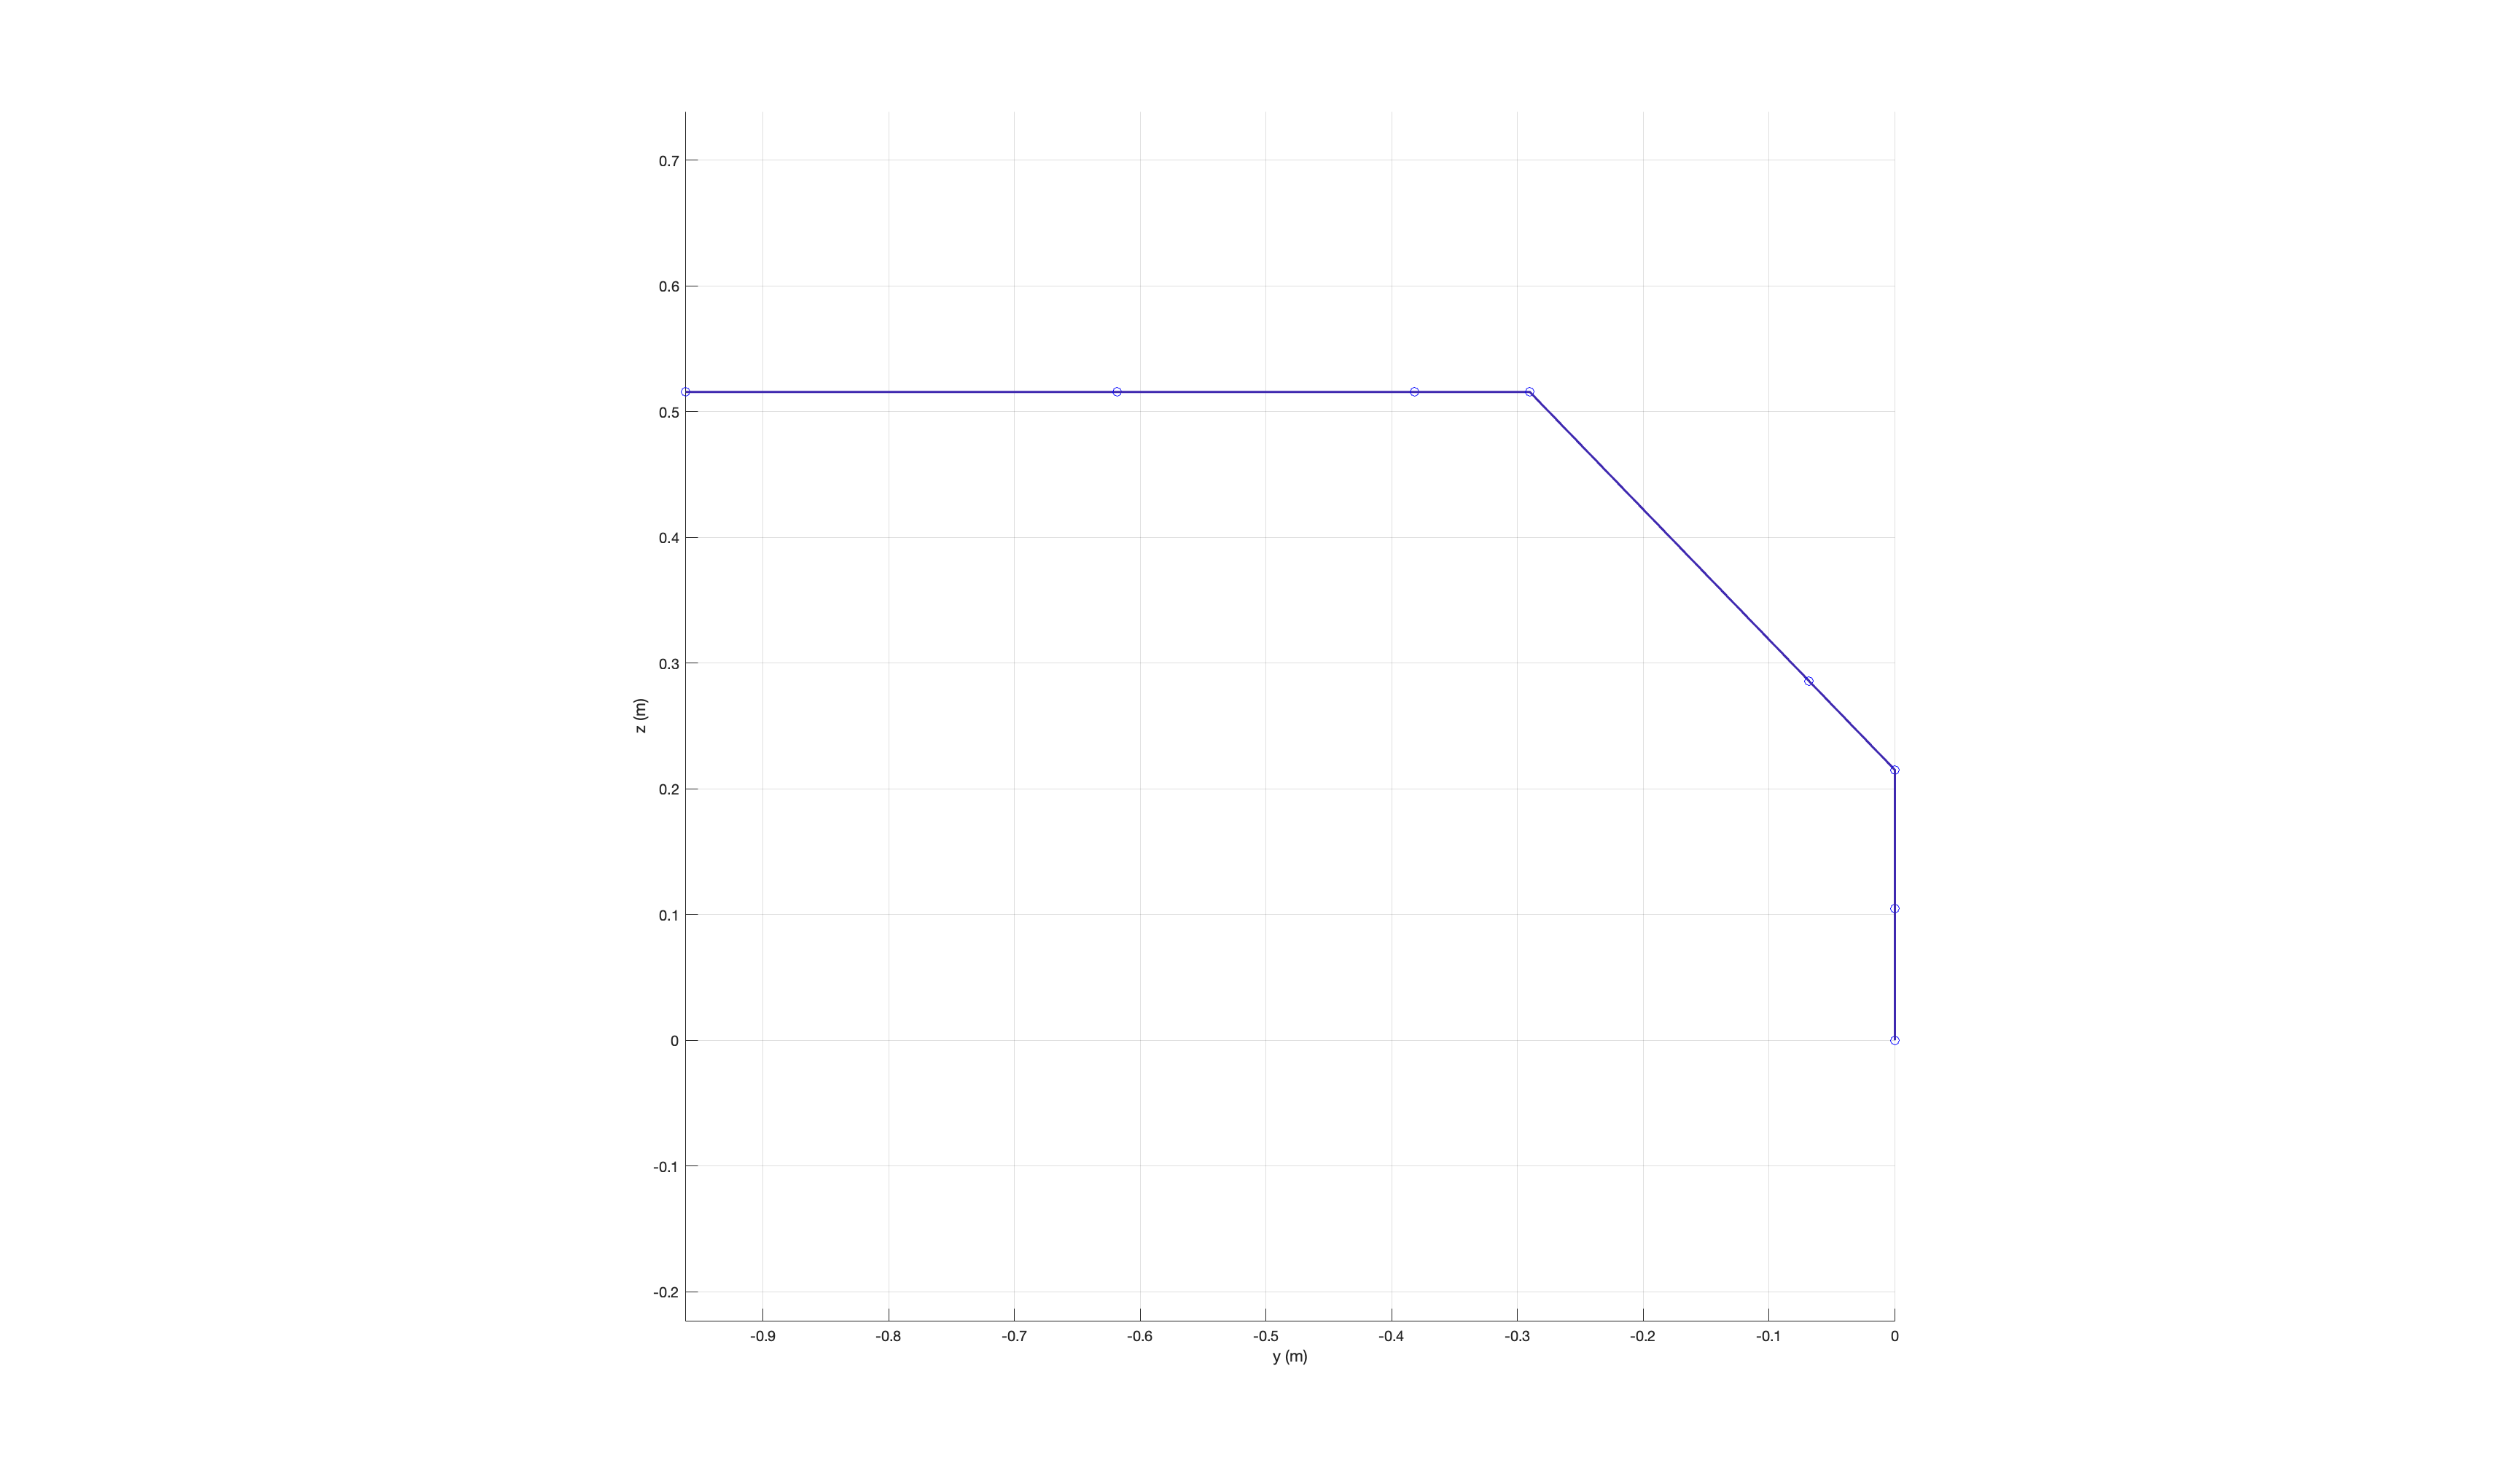
\includegraphics[width=0.75\textwidth]{Resources/FinalConfiguration}
	\caption{Final configuration of the robot during simulated motion on the Cartesian plane $(y, z)$. The measurement units for the three axes are meters.}
	\label{fig::FinalConfiguration}
\end{figure}

